\documentclass[11pt,a4paper]{jsarticle}
\usepackage[dvips]{graphicx}
\usepackage{fancyhdr}
\usepackage{here}
\setcounter{page}{0}
%
\begin{document}

\title{制御工学実験I\hspace{-0.1mm}I\hspace{-0.1mm}I\\ レベル制御(PI制御)}
\author{提出者 \\ 14104064 下松八重 宏太 \\ \\ 共同実験者 \\ 14101028 梶野 翔平 \\ 14104092 中島 美香 \\ 16104311 北山 拓夢}
\date{提出日 \today}



\maketitle
\thispagestyle{empty}
\newpage


\section{目的}
プロセス制御系の制御対象は,一般に,炉,反応装置などの化学プロセスが主である.それらは分布定数系,もしくはムダ時間を含む系であることが多く,その応答時間は数分から数10分にもなり,サーボ系に比べ,極めてゆっくりとしているのが特徴である.ここはプロセス系の一つでああるレベル制御を最も一般的なPID調節器の設計を通じて学習する.
\section{原理}
本実験では,タンク1への流入量$u$を入力とし,タンク2の水位$h_2$を出力とする制御対象の同定を行う.制御対象の伝達関数は以下のような二次遅れ系で表される.
\begin{equation}
 \frac{H_2(s)}{U(s)} = \frac{R_2(s)}{(1+A_1 R_1 s)(1+A_2 R_2 s)}
\end{equation}
ただし,$U(s),H_2(s)$は,それぞれ$u,h_2$のラプラス変換であり,$A_1,A_2$はタンク1,2の断面積,$R_1,R_2$はタンク1,2の流体抵抗である.
しかし,この伝達関数を正確に求めることは難しい.よってこのステップ応答がS字特性を持つことが多いことを利用して伝達関数を1次遅れ+むだ時間系に近似することが出来る.このとき,伝達関数はゲイン$K$,時定数$T$,むだ時間$L$を用いて以下のように表せる.
\begin{equation}
 G_P(s) = \frac{K e^{-Ls}}{Ts+1} 
\end{equation}
S字の作動点近傍で線形化を行い,これと時間軸及び最終値との交点から時定数とむだ時間を求める.
\section{実験方法}
  \subsection{開ループ実験}
   \subsubsection{制御弁}
   流量の制御装置として使用している制御弁の動特性を調べる.制御電流を$4[mA]$から$20[mA]$まで変化させ,その時の定常状態の流量を測定し,電流-流量特性を求める.
   \subsubsection{差圧変換器}
   水位検出器として使用している差圧変換器の動特性を調べる.タンク2の水位を増加させながら,その時の差圧変換器の出力電圧を測定し,水位-出力電圧特性を求める.
   \subsection{開ループ応答}
   制御対象であるタンク1とタンク2にステップ入力を加え,その過渡応答を求める.プログラムの指示にしたがい,制御弁の初期値を$8[mA]$,変化量を$1[mA]$,サンプリング周期を$5[sec]$として測定をする.これより,差圧変換器出力と流量の時間特性を求める.

\subsection{閉ループ実験}
PID調節器を用いて水位を目標水位となるよう調節する. \\
開ループ実験より得られた実験結果から,Ziegler-Nicholsの限界感度法を基づきボード線図を作成しPID調節器のパラメータを決定する.設定するパラメータは以下の通りである.\\
\begin{itemize}
 \item 比例ゲイン$K_P$ \\ 
 \item 積分時間 $T_I$\\
 \item タンク2の目標水位 \\
 \item 差圧変換器のゲイン$D_{gain}$及びオフセット$D_{offset}$ \\
 \item サンプリング周期 \\
\end{itemize}
ここで,差圧変換器の出力電圧$D_out$[V]と水位$H$[cm]の関係を
\begin{equation}
 D_{out} = H \cdot D_{gain} + D_{offset}
\end{equation}
とする.

\section{結果}
  \subsection{開ループ実験}
   \subsubsection{制御弁}
   求めた電流-流量特性を図\ref{fig1}に示す.\\
   図\ref{fig1}において,作動点近傍で線形化した直線も示している.これよりこの制御弁における伝達関数は以下の通りに近似される.

   \begin{figure}
    \begin{center}
     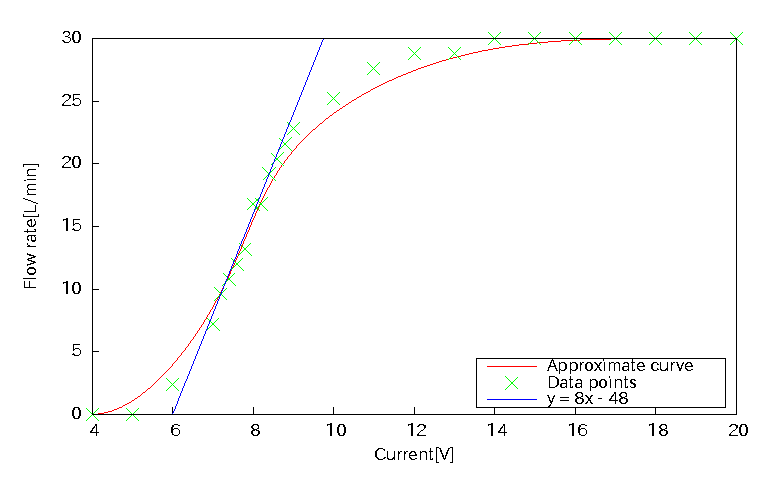
\includegraphics[scale=.7] {./picture/exp1.eps}
     \caption{制御弁の電流-流量特性}
     \label{fig1}
    \end{center}
   \end{figure}

   \begin{equation}
    G_1(s) = \frac{30e^{-6s}}{1+3.75s}
   \end{equation}
   よって電流を入力,流量を出力としたときのブロック線図は図\ref{fig2}のようになる.

   \begin{figure}
    \begin{center}
     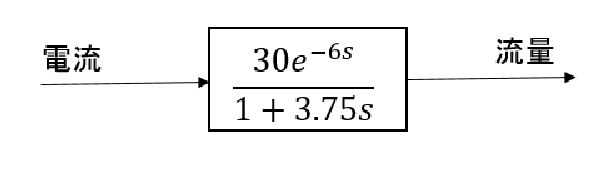
\includegraphics[scale=.7] {./picture/blocks_exp1.eps}
     \caption{制御弁のブロック線図}
     \label{fig2}
    \end{center}
   \end{figure}

   \subsubsection{差圧変換器}
   求めた水位-出力電圧特性及び近似直線を図\ref{fig3}に示す.これよりゲイン$K = 0.016$,オフセット$E = 0.234$となり,水位を入力,出力電圧を出力としたブロック線図は図\ref{fig4}のようになる.

   \begin{figure}
    \begin{center}
     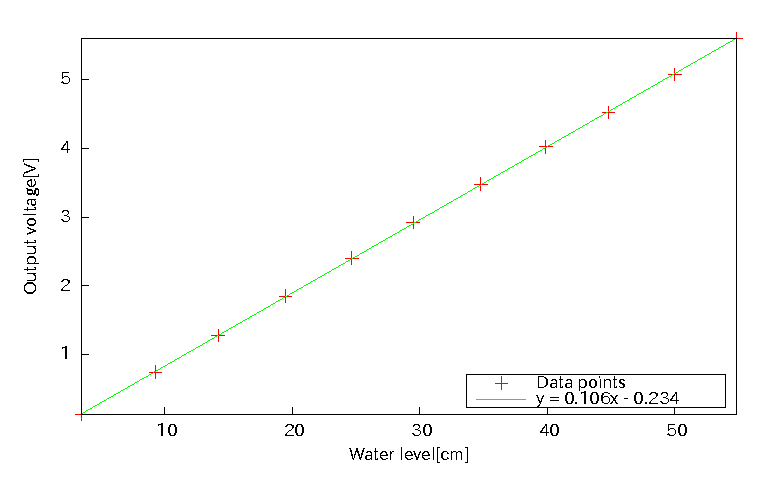
\includegraphics[scale=.7] {./picture/exp2.eps}
     \caption{差圧変換器の水位-出力電圧特性}
     \label{fig3}
    \end{center}
   \end{figure}

   \begin{figure}
    \begin{center}
     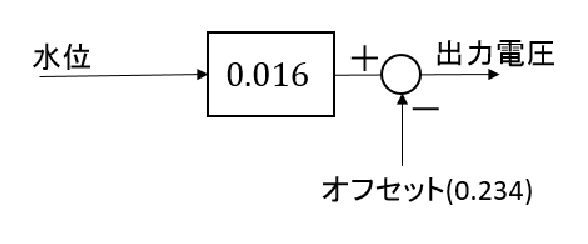
\includegraphics[scale=.7] {./picture/blocks_exp2.eps}
     \caption{差圧変換器のブロック線図}
     \label{fig4}
    \end{center}
   \end{figure}

   \subsubsection{開ループ応答}
   得られたデータより求めた差圧変換器出力と流量の時間特性を図\ref{fig5},図\ref{fig6}に示す.図\ref{fig5}において,図\ref{fig1}と同様に作動点近傍で線形化した直線も示している.図より時定数$T = 69.7$,むだ時間$L = 15.5$,ゲイン$K = 3.65$なので伝達関数は
   \begin{equation}
    G(s) = \frac{3.65e^{-15.5s}}{69.7s+1}
   \end{equation}
   となる.また,流量を入力,出力電圧を出力としたブロック線図は図\ref{fig7}のようになる.

   \begin{figure}
    \begin{center}
     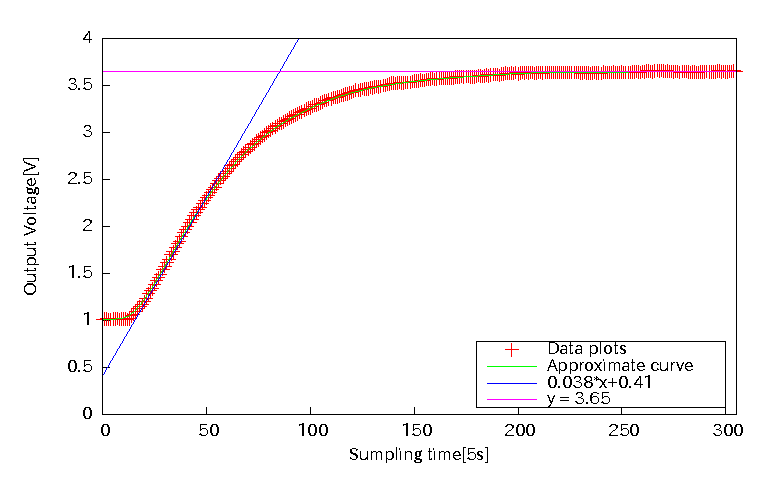
\includegraphics[scale=.7] {./picture/exp3_2.eps}
     \caption{差圧変換器出力の時間特性}
     \label{fig5}
    \end{center}
   \end{figure}

   \begin{figure}
    \begin{center}
     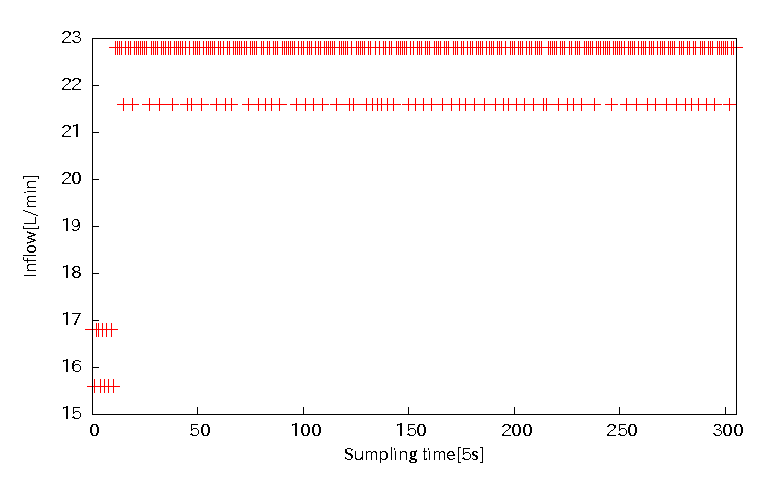
\includegraphics[scale=.7] {./picture/exp3.eps}
     \caption{流量の時間特性}
     \label{fig6}
    \end{center}
   \end{figure}

   \begin{figure}
    \begin{center}
     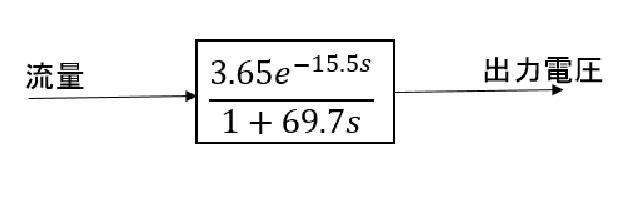
\includegraphics[scale=.7] {./picture/blocks_exp3.eps}
     \caption{ブロック線図}
     \label{fig7}
    \end{center}
   \end{figure}

  \subsection{閉ループ実験}
  開ループ応答実験で得られた伝達関数よりボード線図を作図すると図\ref{fig8}のようになる.
  このとき,位相線図が鋭角に折れ曲がっているが,これはGNUPLOTでボード線図を作図する際,むだ時間要素が入った位相線図は$-\infty$に発散するのでグラフが描けなかったためと考えられる.しかし,$-180$[deg]近傍までは正確に描けているので,このボード線図よりゲイン余裕$g_m$[dB]と位相交点周波数$\omega_c$[Hz]を求める.
  \begin{equation}
   g_m = 6.5 [\rm{dB}], \omega_c = 0.018 [\rm{Hz}]
  \end{equation}
  Ziegler-Nicholsの限界感度法より次の式から,PI制御に用いるパラメータ比例ゲイン$K_P$[dB],積分時間$T_I$[sec]を求める.
  \begin{eqnarray*}
   20 \log_{10}K_C & = & g_m \\
   T_C& = &\frac{2\pi}{\omega_c} \\
   K_P& = &0.45K_C \\
   T_I& = &0.83T_C
  \end{eqnarray*}
  式5より,
  \begin{equation}
   K_P \simeq 2.11 ,T_I \simeq 289
  \end{equation}
  となった.ただし今回の閉ループ実験では以下のパラメータを用いて実験を行った.
  \begin{eqnarray*}
   K_P = 1.123 , T_I = 208.6 , D_{gain} = 0.106 , D_{offset} = -0.234
  \end{eqnarray*}
  また,目標水位は$30$[cm],サンプリング周期を$1$[sec]とした.
  得られた制御弁電流値とタンク2の水位の時間特性を図\ref{fig9},\ref{fig10}に示す.

  \begin{figure}[H]
   \begin{center}
    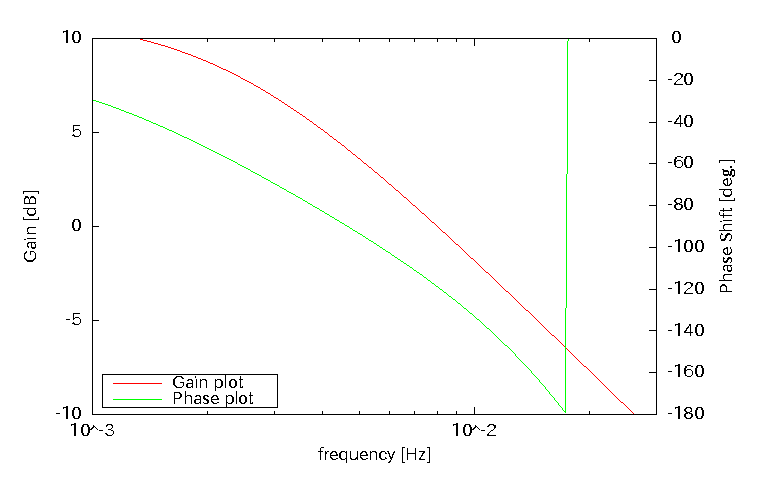
\includegraphics[scale=.7] {./picture/bode2.eps}
    \caption{ステップ応答実験より得られたボード線図}
    \label{fig8}
   \end{center}
  \end{figure}

  \begin{figure}[H]
   \begin{center}
    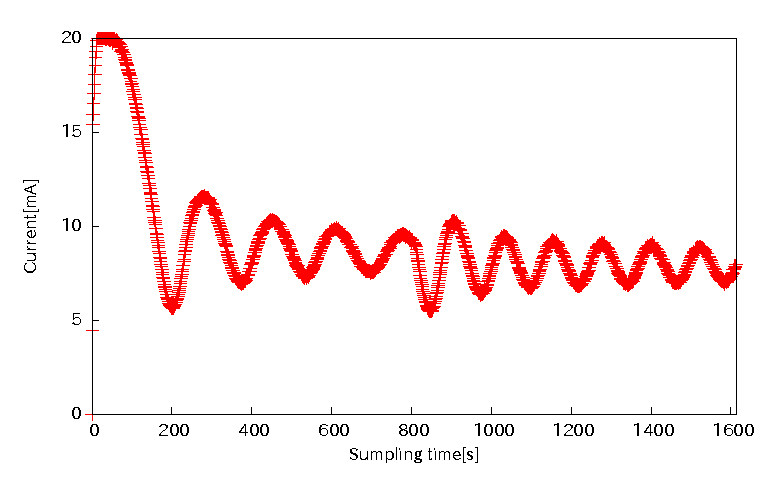
\includegraphics[scale=.7] {./picture/exp4.eps}
    \caption{PI制御を行ったときの制御弁の電流}
    \label{fig9}
   \end{center}
  \end{figure}

  \begin{figure}[H]
   \begin{center}
    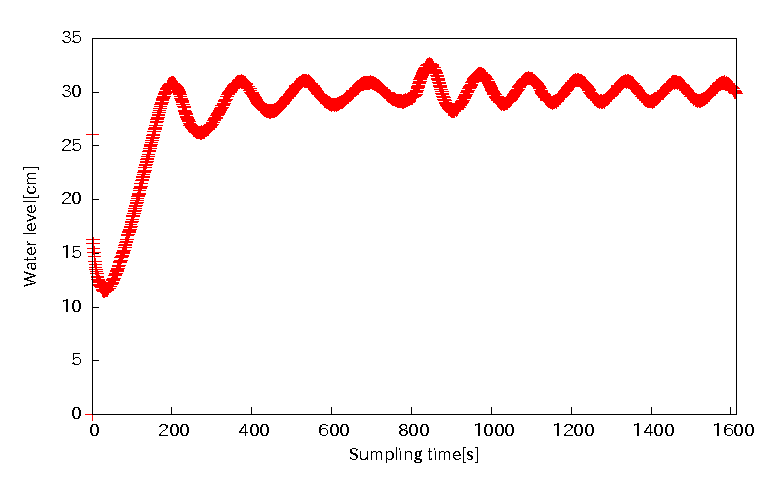
\includegraphics[scale=.7] {./picture/exp4_2.eps}
    \caption{PI制御を行ったときの水位}
    \label{fig10}
   \end{center}
  \end{figure}

 \section{考察及び課題}
  \subsection{閉ループ実験の応答について}
  図\ref{fig9},\ref{fig10}についてみてみる.図\ref{fig9}より,はじめ制御用電流値が最大まで上がった後,最終的には6[mA]から10[mA]程度で振動している.ただし,時間が経つにつれ振動は減衰しているのでさらに時間をかければ定常状態になると考えられる.図\ref{fig10}も目標水位の30[cm]付近で振動しているものの,振動は減衰しているので最終的には定常状態になると考えられる. \\
  今回の実験で2つのグラフが共に整定時間が長くなったのは実験で用いた比例ゲインが大きすぎたためと考えられる.比例制御においては制御偏差を元に操作量を決定するので,その比例ゲインが大きすぎると今回のように振動する.
  \subsection{閉ループ実験におけるボード線図}
  今回行った閉ループ実験におけるブロック線図は図\ref{fig11}である.よって制御系全体の伝達関数は
  \begin{equation}
   G(s) = K_P(1 + \frac{1}{T_I s}) \cdot \frac{K e^{-Ls}}{Ts + 1}
  \end{equation}
  となる.これよりボード線図を作図すると図\ref{fig12}のようになる.

  \begin{figure}
   \begin{center}
    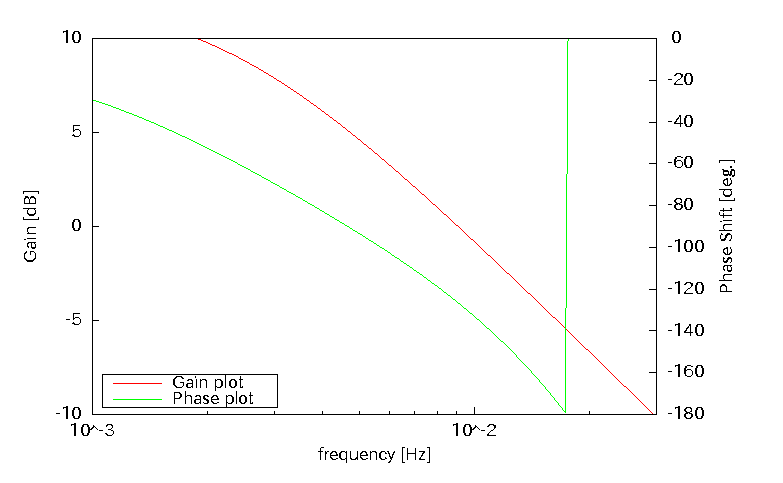
\includegraphics[scale=.7] {./picture/bode3.eps}
    \caption{閉ループ実験におけるボード線図}
    \label{fig12}
   \end{center}
  \end{figure}

  図\ref{fig12}からゲイン余裕$g_m$と位相余裕$\phi_m$を求めると,
  \begin{eqnarray*}
   g_m \simeq 5.56[\rm{dB}] \\
   \phi_m \simeq 40[\rm{deg}]
  \end{eqnarray*}
  となった.
  \begin{figure}
   \begin{center}
    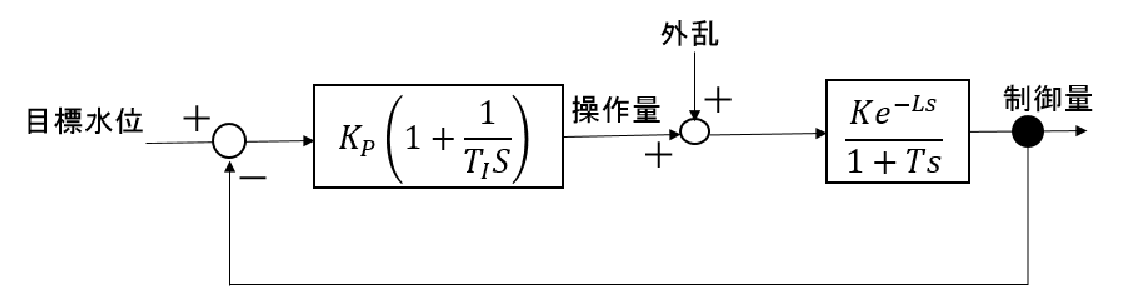
\includegraphics[scale=.7] {./picture/blocks_exp4.eps}
    \caption{プロセス制御系}
    \label{fig11}
   \end{center}
  \end{figure}

\subsection{$\rm{PID}$制御の場合}
今回の実験ではPI制御を用いてプロセス系の制御を行った.ここに微分制御を足したPID制御で制御を行う場合を考える.微分制御では制御偏差の変化量に応じて操作量を決定するので,変化量を抑え応答が振動するのを抑制する.よって,今回のように応答が振動的なものがより早く定常状態になると考えられる.

\subsection{その他の$\rm{PID}$調節器のパラメータ決定法}
今回用いたZiegler-Nicholsの限界感度法の他のPID調節器のパラメータ決定法として,CHR法がある.これは設定変化値及び外乱に対して,それぞれ「オーバーシュートなし」及び「オーバーシュート20\%」の場合に最も応答が早くなるパラメータを求めている.CHR法においても,制御系は一次遅れ+むだ時間系で表されており,そのゲインと時定数,むだ時間からパラメータを決定する. \\
また,試行錯誤法をとる事も出来る.これはその名の通り各パラメータを試行錯誤で求めていく手法である.これは1つの手法としては認められないかもしれないが,PID制御の利点の1つとして現場でパラメータの調整ができることにある.[1]


\begin{thebibliography}{1}
 \bibitem[1] 山本ら,”PID制御の基礎と応用 第2版”,朝倉書店,pp.93-94,2005
\end{thebibliography}

\newpage
\setcounter{page}{1}
%\renewcommand{\thepage}{\thepage}
\pagestyle{fancy}
\renewcommand{\headrulewidth}{0.0pt}
\rhead{再\thepage}
\lhead{}
\cfoot{}

\section{実験装置}
今回の実験で使用したタンクの概要を図\ref{fig14}に示す.図中の各文字は前
述の通りである.
\begin{figure}[b]
 \begin{center}
  \includegraphics[scale=.5]{./picture/tank.eps}
  \caption{レベル系の実験装置}
  \label{fig14}
 \end{center}
\end{figure}


\section{システム同定の見直し}
図\ref{fig5}より横軸の単位は[5sec]なので,時定数とむだ時間を求めると
\begin{eqnarray*}
T & = & 15.5 \cdot 5 \\
  & = & 77.5 \\
L & = & 69.7 \cdot 5 \\
  & = & 348.5
\end{eqnarray*}
となる.よって,伝達関数は

\begin{equation}
  G(s) = \frac{2.65e^{-77.5s}}{348.5s+1} 
\end{equation}
となる.これより,ボード線図を求めると,図\ref{fig13}のようになる.

\begin{figure}[H]
 \begin{center}
  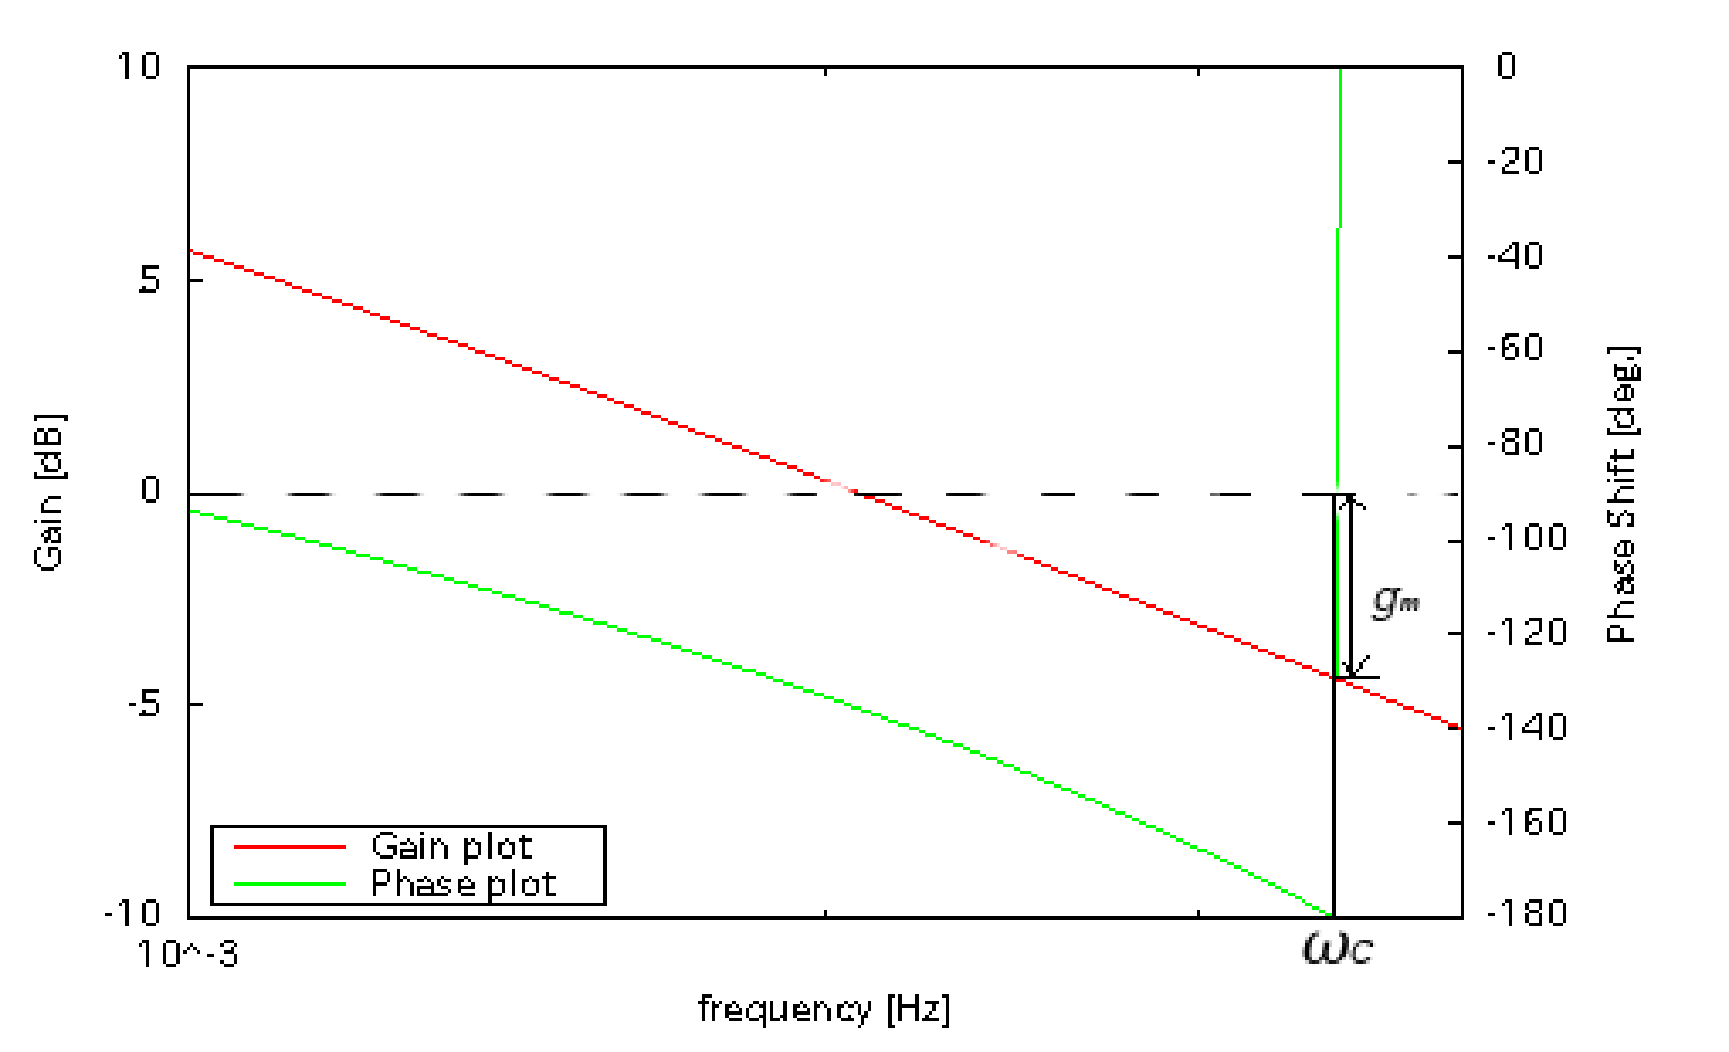
\includegraphics[scale=.5]{./picture/bode4.eps}
  \caption{ボード線図}
  \label{fig13}
 \end{center}
\end{figure}

ボード線図より,ゲイン余裕$g_m$,位相交点周波数$\omega_c$は
\begin{equation}
 g_m = 4.4, \omega_c = 0.035 \nonumber
\end{equation}
となるので,比例ゲイン$K_P$と積分時間$T_I$は
\begin{eqnarray}
K_P & = & 0.45 \cdot 10^{\frac{g_m}{20}} \\
    & = & 0.75 \\
T_I & = & 0.83 \cdot \frac{2\pi}{\omega_c} \\
    & = & 149 
\end{eqnarray}
となった.


 \newpage
\section{$\rm{CHR}$法について}
CHR法ではゲイン$K$,時定数$T$,むだ時間$L$を用いて次の式よりPI制御の各パラメータを求める.
\subsection{オーバーシュートなしの時}
\begin{eqnarray*}
 K_P & = & 0.35 \cdot \frac{T}{KL} \\
 T_I & = & 1.2T
\end{eqnarray*}
\subsection{オーバーシュート 20$\%$の時}
\begin{eqnarray*}
 K_P & = & 0.6 \frac{T}{KL} \\
 T_I & = & T
\end{eqnarray*}

\newpage
\setcounter{page}{1}
\pagestyle{fancy}
\renewcommand{\headrulewidth}{0.0pt}
\rhead{再々\thepage}
\lhead{}
\cfoot{}
 
\section{2次遅れ系の近似について}
図\ref{fig1},図\ref{fig5}のような2次遅れ系を1次遅れ系とむだ時間で近似す
るとき,2次遅れ系のグラフより変曲点で接線を引くことで線形化し近似してい
る.


\end{document}








